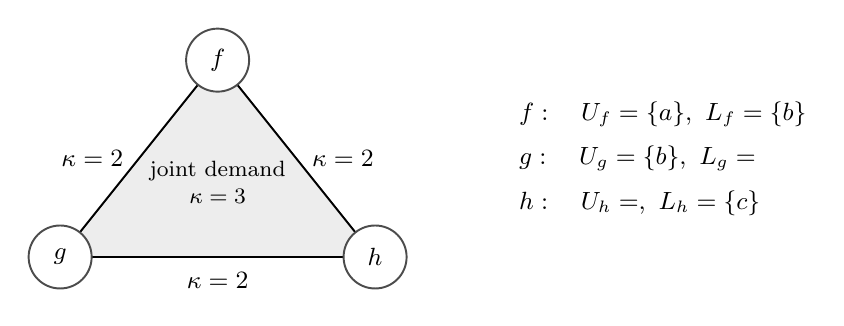
\begin{tikzpicture}[font=\small,every path/.style={line width=.7pt},
 world/.style={circle,draw=black!70,fill=white,minimum size=8mm,inner sep=1pt}]
\fill[black!7] (0,2.5) -- (-2,0) -- (2,0) -- cycle;
\draw (0,2.5) -- node[left,xshift=-2pt] {$\kappa=2$} (-2,0);
\draw (0,2.5) -- node[right,xshift=2pt] {$\kappa=2$} (2,0);
\draw (-2,0) -- node[below,yshift=-2pt] {$\kappa=2$} (2,0);
\node[world] at (0,2.5) {$f$};
\node[world] at (-2,0) {$g$};
\node[world] at (2,0) {$h$};
\node[align=center,font=\footnotesize] at (0,.95) {joint demand\\$\kappa=3$};
\node[anchor=west,align=left] at (3.7,1.25) {
  $f:\quad U_f=\{a\},\ L_f=\{b\}$\\[5pt]
  $g:\quad U_g=\{b\},\ L_g=\varnothing$\\[5pt]
  $h:\quad U_h=\varnothing,\ L_h=\{c\}$};
\end{tikzpicture}
